\chapter{Introduction}
% ============================================================
% Genesis, Definition, Orientation, Motivation — harmonized with Chapter 0
% (Diamond 20/10; extended+++ final synthesis, line-edited, with targeted enrichments)
% ============================================================

% ------------------------------------------------------------
% Programmatic epigraph / manifesto
% ------------------------------------------------------------
\begin{center}
\emph{``Every new mathematical discipline begins not with technique but with the sighting of a paradox---a stubborn phenomenon that resists existing frames. Lithomathematics begins with the paradox of the internal wall.''}
\end{center}

\section{Genesis of Lithomathematics}\label{sec:genesis}

\subsubsection*{1.1.1 The Observational Paradox}
\paragraph{The Paradox of the Obvious.}
Internal \emph{hard walls} are ubiquitous: fracture planes in rock, barrier layers in composites, cellular membranes, microstructured partitions in nanodevices.
They divide a domain into chambers that do not communicate across the wall.
Yet for decades these interfaces remained \emph{spectral ghosts}: omnipresent in applications, nearly absent in canonical spectral geometry.
This monograph addresses that systematic gap by placing \emph{internal Dirichlet walls}—$C^2$ interior hypersurfaces $\Gamma\subset M$ with $u|_\Gamma=0$—at the center of analysis.

\subsubsection*{1.1.2 Formal Definition}
\paragraph{Definition (Lithomathematics).}
\emph{Lithomathematics} is the spectral–geometric analysis of Laplace–type operators on compact Riemannian manifolds $(M,g)$ \emph{sliced} by internal Dirichlet hypersurfaces $\Gamma$ (``hard walls'').
Its operator–theoretic core is the \emph{litho–Laplacian} $L_\Gamma$, introduced in \textbf{Definition~\ref{def:litho-Laplacian}} as the self–adjoint operator associated with the Dirichlet form on $H^1_0(M;\partial M\cup\Gamma)$ (see also \textbf{Remarks~\ref{rem:trace-continuity}, \ref{rem:components}}).
All short–time statements about the heat trace are made in the diffusive scale $\tau$ and use the expansion of \textbf{Definition~\ref{def:heat-expansion}} together with the universality \textbf{Convention~\ref{conv:universality}}.

\subsubsection*{1.1.3 Terminology and Conventions}
\paragraph{Etymology.}
The term derives from Greek \emph{lithos} (stone, rock): internal “stone–like’’ obstructions are treated as first–class spectral objects, distinct from soft walls (Neumann) and transmissive seams (Robin/impedance).

\paragraph{What lithomathematics is \emph{not}.}
It is not exterior scattering (no radiation to infinity), not transmission theory (no cross–interface coupling), not a boundary perturbation (the wall is \emph{interior}), and not a soft–wall/Neumann model (no–flux $\neq$ vanishing field).
The novelty is a \emph{parameter–free interior universal law} produced by a non–transmitting Dirichlet wall.

\paragraph{Terminological conventions (physics–compatible).}
\begin{itemize}
  \item \emph{Hard wall} $\equiv$ internal Dirichlet constraint $u|_\Gamma=0$.
  \item \emph{Heat:} Dirichlet acts as an \emph{isothermal sink} on $\Gamma$ (not “no–flux”, which is Neumann).
  \item \emph{Waves/quantum:} Dirichlet is a perfectly reflecting wall; the field vanishes on $\Gamma$, reflection has phase $\pi$.
\end{itemize}

\paragraph{Notation and linkage to Chapter~0.}
We use $\vol_{k}(\cdot)$ for $k$–dimensional Riemannian measure, $R=\mathrm{diam}_g(M)$, $\vec H_\Gamma$ for the mean curvature vector of $\Gamma$, and $S^*(X)$ for the unit cosphere bundle.
Standing assumptions (reach, transversality, piecewise $C^2$) and notational conventions are fixed in Chapter~0 (\S\ref{sec:definitions}).

\paragraph{Central Problem.}
Establish a universal, curvature–independent \emph{interior} contribution $a_\Gamma$ to the heat trace (and to Weyl’s counting law), prove its stability, identify the first geometry–dependent layer beyond universality, and link global remainders to reflecting dynamics under a mixing hypothesis.

\subsubsection*{1.1.4 Canonical Examples: From Geology to Nanodevices}
\begin{itemize}
  \item \textbf{Geological fault as a wave barrier.} A seismic displacement field $u$ in rock encounters a sharp, impermeable fracture $\Gamma$; slip surfaces impose $u|_\Gamma=0$ along the crack faces.
  \item \textbf{Impermeable membrane in a microfluidic chip.} A concentration $c$ diffuses in a chamber bisected by a lipid bilayer; perfect containment is modeled by $c|_\Gamma=0$.
  \item \textbf{Quantum dot with hard confinement.} An electron in a heterostructure is trapped in a subdomain $U_j$; potential walls idealized as Dirichlet $\Gamma$ enforce the vanishing of the wavefunction on the interface.
\end{itemize}
These are not perturbations of a boundary problem; they are \emph{new spectral objects} with two–sided functional singularity supported on $\Gamma$.

\medskip

\section{Principal Contributions}\label{sec:contrib}

\paragraph{1. The Litho–Laplacian $L_\Gamma$.}
A canonical self–adjoint operator for manifolds with internal Dirichlet walls, rigorously founded via the closed form on $H^1_0(M;\partial M\cup\Gamma)$ (Chapter~0, \textbf{Definition~\ref{def:litho-Laplacian}}; \textbf{Remark~\ref{rem:components}}).

\paragraph{2. Universal Interior Law.}
A curvature–independent interior surface coefficient $a_\Gamma$ at order $\tau^{-(d-1)/2}$, fully analogous to the exterior Dirichlet term but supported on $\Gamma$ (Chapter~0, \textbf{Definition~\ref{def:heat-expansion}}, \textbf{Convention~\ref{conv:universality}}).

\paragraph{3. Dimensionless Geometric Complexity.}
A scale–free invariant $\kappa(\Gamma)$ bundling fragmentation, area and bending, controlling constants in non–universal layers without affecting the universal coefficient (Chapter~0, \textbf{Definition~\ref{def:complexity}}).

\paragraph{4. Spectral–Dynamical Bridge.}
Under the reflecting–flow mixing hypothesis $H_{\mix}^{\heartsuit}$ one transfers correlation decay into refined remainder estimates for counting functions (Chapter~0, \textbf{Hypothesis~\ref{hyp:mixing-hermetic}}).

\paragraph{5. Architectonic Pipeline.}
A systematic pathway
\[
\mathrm{SA}\;\Longrightarrow\;\mathrm{FA}\;\Longrightarrow\;\mathrm{GEO}\;\Longrightarrow\;\mathrm{UNI}\;\ (\Longrightarrow\;\mathrm{DYN})
\]
that isolates the universal interior law from geometric regularity and functional setup, and (optionally) transfers dynamical mixing into global remainder bounds.

\medskip

\section{Historical Context}\label{sec:history}

The prehistory of lithomathematics spans four mature traditions. Each attained depth in its domain, yet all left the same blind spot: smooth \emph{interior} hard walls as primary spectral objects.

\subsection*{(I) Boundary paradigm (1960s–1980s): universality anchored at the exterior}
Seeley, Greiner, McKean–Singer, Gilkey developed heat asymptotics for smooth external boundaries; Kac’s question “Can one hear the shape of a drum?” catalyzed the field.
The boundary term
\[
a_{1/2}(\partial M) \;=\; -\tfrac14(4\pi)^{-(d-1)/2}\,\vol_{d-1}(\partial M)
\]
became a paradigm of universality at this order; interior partitions lie outside the boundary calculus.
\emph{Limitation:} classical boundary parametrices are inherently \emph{one–sided}; a two–sided interior hypersurface $\Gamma$ violates the single–collar assumption.

\subsection*{(II) Singular stratification (1980s–2000s): metric singularities, not functional ones}
The Cheeger–Mazzeo–Melrose program mastered cones/edges/cusps.
A $C^2$ interior wall with Dirichlet constraint is geometrically smooth yet \emph{functionally} singular; it falls outside conic/edge taxonomies.
\emph{Limitation:} functional walls without metric singularity are invisible to purely metric stratifications.

\subsection*{(III) Transmission/impedance theory: coupling as principle}
Grisvard and successors built PDE theory for transmissive interfaces.
Leading coefficients depend on interface parameters; universality is lost by construction.
Non–transmitting Dirichlet walls are excluded.
\emph{Limitation:} parameter–dependence precludes a parameter–free universal surface law.

\subsection*{(IV) Billiards and dynamics: reflections at external boundaries}
From Sinai/Bunimovich to Chernov–Markarian and the spectral–dynamical bridge of Safarov–Vassiliev, billiards illuminated mixing and spectra.
Internal reflecting walls, however, were not treated as \emph{primary spectral objects} linked to local heat asymptotics.
\emph{Limitation:} dynamics inform remainders but do not manufacture the missing interior surface coefficient.

\paragraph{Timeline of related developments.}
1966: Kac; 1971: Greiner; 1985: Grisvard; 1995: Gilkey; 1997: Safarov–Vassiliev; 2006: Chernov–Markarian; 2020s: lithomathematics synthesizes these strands around internal hard walls.

\paragraph{Why Now?}
(i) \emph{Technology} realizes hard–wall confinement at micro/nano scales; (ii) \emph{Analysis} matured (reach geometry, interior parametrices, Tauberian techniques, quantitative mixing); (iii) \emph{Applications} demand parameter–free universal laws beyond exterior geometry.

\medskip

\section{From Classical to New Phenomena}\label{sec:classical-new}

\paragraph{Three paradigms in contrast (with physical readings).}
\begin{center}
\renewcommand{\arraystretch}{1.15}
\begin{tabular}{|l|l|l|l|l|l|}
\hline
\textbf{Paradigm} & \textbf{Condition} & \textbf{Order} & \textbf{Coefficient} & \textbf{Universality} & \textbf{Physical reading} \\
\hline
Boundary (Dir) & $u|_{\partial M}=0$ & $\tau^{-(d-1)/2}$ & $-\tfrac14(4\pi)^{-(d-1)/2}\vol(\partial M)$ & yes & exterior capacity deficit \\
\hline
Boundary (Neu) & $\partial_\nu u|_{\partial M}=0$ & $\tau^{-(d-1)/2}$ & $+\tfrac14(4\pi)^{-(d-1)/2}\vol(\partial M)$ & yes & no–flux (soft wall) \\
\hline
Transmission & $[u]=0,\ [\partial_\nu u]=\kappa u$ & $\tau^{-(d-1)/2}$ & depends on $\kappa$ & no & impedance–driven \\
\hline
Lithomathematics & $u|_{\Gamma}=0$ (internal) & $\tau^{-(d-1)/2}$ & $-\tfrac14(4\pi)^{-(d-1)/2}\vol(\Gamma)$ & yes & interior hard–wall deficit \\
\hline
\end{tabular}
\end{center}

\noindent The distinctive phenomenon is the \emph{interior universal law}
\[
a_\Gamma \;=\; -\tfrac14(4\pi)^{-(d-1)/2}\,\vol_{d-1}(\Gamma),
\]
entirely analogous to the exterior Dirichlet term yet arising \emph{strictly from an internal wall}.
The negative sign corresponds physically to a reduction of accessible modes (quantum/acoustic) or, in the heat picture, to a decrease of effective heat capacity due to the internal barrier.\footnote{\textbf{Method of images (local sketch).}
In flat Fermi coordinates $(x',x_d)$ with $\Gamma=\{x_d=0\}$, the local Dirichlet kernel is
$H^{\rm Dir}\!\approx H^{\mathbb{R}^d}(x-y;\tau)-H^{\mathbb{R}^d}(x-\tilde y;\tau)$, $\tilde y=(y',-y_d)$.
Integrating the deficit in a tubular collar and patching by a partition of unity yields the density $-\frac14(4\pi)^{-(d-1)/2}\mathrm{area}(\Gamma)\,\tau^{-(d-1)/2}$.
This is rigorously justified by the parametrix in Ch.~3 (see Chapter~0, \textbf{Definition~\ref{def:heat-expansion}}, \textbf{Convention~\ref{conv:universality}}).}

\paragraph{Dimensional check (sanity).}
The interior term has density $-(4\pi)^{-(d-1)/2}/4$ per unit $(d\!-\!1)$–area, so
\[
[a_\Gamma]=[\mathrm{area}]\cdot[\tau^{-(d-1)/2}] \;=\; L^{d-1}\cdot L^{-(d-1)} \;=\; 1,
\]
consistent with a dimensionless coefficient in the heat trace expansion.

\medskip

\section{Orientation and Scope}\label{sec:orientation}

Lithomathematics rests on five interlocking pillars (as formalized in Chapter~0):

\begin{itemize}
  \item \textbf{(SA) Geometric regularity.} Piecewise $C^2$ boundaries and wall, positive reach and transversality (\emph{Standing Assumptions}, \textbf{Remark~\ref{rem:relative-reach}}).
  \item \textbf{(FA) Functional analysis.} $L_\Gamma$ as in \textbf{Definition~\ref{def:litho-Laplacian}}; trace continuity (\textbf{Remark~\ref{rem:trace-continuity}}); componentwise spectral splitting (\textbf{Remark~\ref{rem:components}}).
  \item \textbf{(GEO) Geometric complexity.} Scale–free invariant $\kappa(\Gamma)$ in \textbf{Definition~\ref{def:complexity}}.
  \item \textbf{(UNI) Universal interior law.} Leading interior density at $\tau^{-(d-1)/2}$ (Ch.~3).
  \item \textbf{(DYN) Dynamical regime (optional).} Reflecting flow and $H_{\mix}^{\heartsuit}$ (\textbf{Hypothesis~\ref{hyp:mixing-hermetic}}) for refined remainders.
\end{itemize}

\paragraph{Logical cascade (necessity, not choice).}
(SA)$\Rightarrow$(FA)$\Rightarrow$(GEO)$\Rightarrow$(UNI); (DYN) bridges to global remainders (Figure~\ref{fig:cascade}).

\begin{figure}[t]
\centering
\fbox{\parbox{0.92\textwidth}{
\textbf{Figure 1.1 (Logical cascade).}
SA (reach, $C^2$) $\Rightarrow$ FA (Friedrichs $L_\Gamma$, trace framework) $\Rightarrow$ GEO ($\kappa(\Gamma)$, scale–free control) $\Rightarrow$ UNI (interior universal law).
Optional DYN ($H_{\mix}^{\heartsuit}$) $\Rightarrow$ Tauberian transfer $\Rightarrow$ improved global remainders.
% (A TikZ block-flow version is provided in the source repository for camera-ready figures.)
}}
\label{fig:cascade}
\end{figure}

% ------------------------------------------------------------
% Working hypotheses (explicit, for cross-reference)
% ------------------------------------------------------------
\subsection*{Working Hypotheses (for cross-reference)}
\begin{description}
  \item[H1 (Interior Universality).] Under (SA), the surface density at order $\tau^{-(d-1)/2}$ equals $-\frac{1}{4}(4\pi)^{-(d-1)/2}$ per unit $(d\!-\!1)$–area on $\Gamma$, independent of curvature and material parameters.
  \item[H2 (Stability).] $a_\Gamma$ is stable under $C^2$ perturbations preserving positive reach and transversality, with locality of the coefficient.
  \item[H3 (Complexity Control).] Non–universal constants in local expansions and global remainders are governed by a scale–free invariant $\kappa(\Gamma)$.
  \item[H4 (Dynamical Transfer).] If $H_{\mix}^{\heartsuit}$ holds for the reflecting flow, then correlation decay yields sub–Weyl improvements $R(\lambda)=O(\kappa(\Gamma)\lambda^{(d-2)/2-\alpha})$ for some $\alpha>0$.
\end{description}

\medskip

\section{Conceptual Novelty}\label{sec:novelty}

\begin{enumerate}
  \item \textbf{Dirichlet slicing.} Treating $\Gamma$ as a non–transmitting wall yields the orthogonal decomposition
  \[
  L^2(M)=\bigoplus_{j} L^2(U_j)
  \]
  across connected components $U_j$ of $M\setminus\Gamma$ (Figure~\ref{fig:decomp}), with a clean microlocal picture near $\Gamma$ and the universal interior density $a_\Gamma$ at order $\tau^{-(d-1)/2}$.
  At the level of propagation, this implements a “no cross–talk’’ principle: singularities do not transmit across $\Gamma$.
  \item \textbf{Scale–free complexity.} $\kappa(\Gamma)$ (\textbf{Definition~\ref{def:complexity}}) bundles fragmentation, area and bending into a dimensionless control for non–universal constants, leaving universal coefficients untouched.
\end{enumerate}

\paragraph{Microlocal propagation near \texorpdfstring{$\Gamma$}{Gamma}.}
At smooth interior points of $\Gamma$ the wave front set reflects specularly: incoming covectors $(x,\xi)$ with $\xi\cdot\nu<0$ map to
\[
(x,\xi)\ \longmapsto\ \big(x,\ \xi-2(\xi\cdot\nu)\nu\big),
\]
with no cross–interface transmission of singularities. Diffraction appears only at corner/edge strata
$\partial\Gamma\cup(\Gamma\cap\partial M)$ and does \emph{not} affect the leading interior surface density at order $\tau^{-(d-1)/2}$.

\paragraph{Why the universality is not obvious (counter–intuition).}
It is tempting to expect that strong curvature of $\Gamma$ should alter the \emph{leading} surface density. Lithomathematics proves otherwise: at order $\tau^{-(d-1)/2}$ only \emph{area} matters. A thin but long internal wall can dominate a short highly curved wall, despite the latter’s geometric complexity. Curvature first appears at order $\tau^{-(d-2)/2}$ via Seeley–DeWitt invariants; thus, geometric bending is \emph{subleading}.

\begin{figure}[t]
\centering
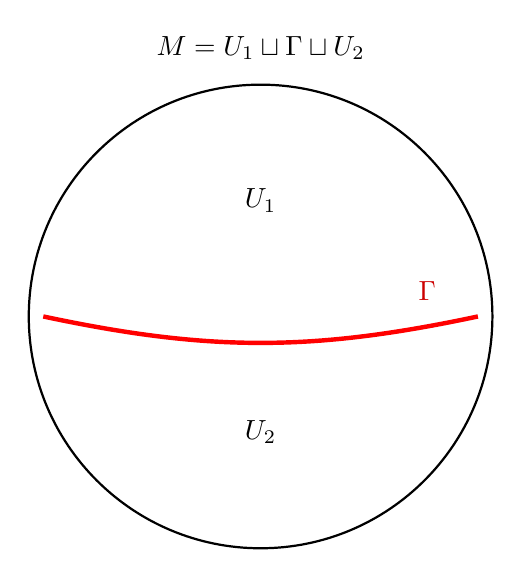
\begin{tikzpicture}[scale=0.92]
  % Domain M
  \draw[thick] (0,0) circle (3.2cm);
  % Internal wall Gamma
  \draw[ultra thick, red] (-3.0,0) to[bend right=12] (3.0,0);
  % Labels
  \node at (0,1.6) {$U_1$};
  \node at (0,-1.6) {$U_2$};
  \node[red!80!black] at (2.3,0.35) {$\Gamma$};
  \node at (0,3.7) {$M = U_1 \sqcup \Gamma \sqcup U_2$};
\end{tikzpicture}
\caption{\textbf{Figure 1.2 (Interior decomposition).} Orthogonal splitting $L^2(M)=L^2(U_1)\oplus L^2(U_2)$ induced by an internal Dirichlet wall $\Gamma$; lithomathematics treats $\Gamma$ as a \emph{primary spectral object}.}
\label{fig:decomp}
\end{figure}

\medskip

\section{Illustrative Perspective}\label{sec:perspective}

\subsection*{Heat: isothermal interior sinks.}
\[
\partial_\tau u=\Delta u,\qquad u|_{\partial M\cup\Gamma}=0.
\]
The interior term $a_\Gamma$ encodes the capacity deficit $\propto \vol_{d-1}(\Gamma)$, independent of curvature at leading order.

\subsection*{Waves/quantum: perfectly reflecting walls.}
\[
(\partial_\tau^2+L_\Gamma)u=0,\qquad u|_\Gamma=0.
\]
Reflection has phase $\pi$. Hilbert space decomposes across chambers; spectral statistics shift; mixing informs remainders (DYN).

\subsection*{Statistical-physics reading: mode-count and entropy.}
At leading order, the area law $a_\Gamma\propto -\mathrm{area}(\Gamma)$ equals the \emph{mode deficit} induced by perfectly reflecting interior constraints.
In thermal ensembles this manifests as a reduction of effective heat capacity and entropy at small times/large frequencies, consistent with universal, material–independent behavior.

\subsection*{Applied prototype: layered composite.}
For $M\subset\mathbb{R}^3$ with a single impermeable layer $\Gamma$ and Dirichlet on $\partial M\cup\Gamma$,
\[
\Tr(e^{-\tau L_\Gamma})=a_0\tau^{-3/2}+\big(a_{1/2}(\partial M)+a_\Gamma(\Gamma)\big)\tau^{-1}+O(\tau^{-1/2}),
\quad
a_\Gamma(\Gamma)=-\frac14(4\pi)^{-1}\mathrm{area}(\Gamma).
\]

\medskip

\section{Proof Strategy Overview (methods without proofs)}\label{sec:proof-strategy}

\paragraph{Parametrix (UNI).}
Local flattening and rescaling in a tubular collar (reach $>$0) produce the interior density $a_\Gamma$; corner/edge strata yield displaced/log terms but do not alter the smooth interior density (cf.\ \textbf{Definition~\ref{def:heat-expansion}}, \textbf{Remark~\ref{rem:corners}}).

\paragraph{Seeley–DeWitt (GEO).}
Curvature invariants enter at $\tau^{-(d-2)/2}$ (\textbf{Remark~\ref{rem:seeley-dewitt}}); constants are organized via $\kappa(\Gamma)$.

\paragraph{Tauberian transfer (DYN).}
Assuming $H_{\mix}^{\heartsuit}$ (\textbf{Hypothesis~\ref{hyp:mixing-hermetic}}), decay of correlations yields cancellations in oscillatory integrals, giving
\[
R(\lambda)=O\!\big(\kappa(\Gamma)\,\lambda^{(d-2)/2-\alpha}\big),\quad \alpha>0.
\]
(DYN is an optional accelerator; it does not affect $a_\Gamma$.)

\paragraph{Methodological innovation (synthetic method).}
Lithomathematics synthesizes three traditions around $L_\Gamma$: (i) geometric measure theory (reach, tubular parametrizations), (ii) functional analysis on nonsmooth partitions (trace theory and Friedrichs extensions on $M\setminus\Gamma$), (iii) spectral dynamics and Tauberian machinery (heat–wave correspondence, cancellation via mixing). The novelty lies in their systematic integration to isolate a parameter–free interior law and to organize next–order effects.

\paragraph{Techniques at a glance (toolbox).}
\begin{itemize}
  \item Interior Dirichlet parametrices in Fermi charts; reflection method; uniform error control by positive reach.
  \item Tauberian bridge \`a la Safarov–Vassiliev (heat–wave correspondence; Abelian bounds).
  \item Stationary phase for oscillatory integrals; elimination of grazing sets; microlocal propagation with specular reflection.
\end{itemize}

\medskip

\section{Scope, Limitations, and Exact Boundaries}\label{sec:scope}

\paragraph{In scope.}
Compact $(M,g)$; piecewise $C^2$ boundary and interior wall; positive reach; Dirichlet on $\partial M\cup\Gamma$ (cf.\ (SA) and \textbf{Remark~\ref{rem:relative-reach}}).
Local universality is asserted away from $\partial\Gamma\cup(\Gamma\cap\partial M)$ (\textbf{Remark~\ref{rem:local-universal-density}}).

\paragraph{Out of scope (by design).}
Transmission/Robin (parameter–dependent leading terms), noncompact manifolds with essential spectrum, cusps/self–intersections (reach fails).
This exclusion protects the universality claim.

\paragraph{Why \texorpdfstring{$C^2$}{C2} (minimal regularity for universality).}
$C^2$ regularity ensures a well–defined second fundamental form and uniform tubular coordinates (positive reach), needed for the interior parametrix with controlled errors. At merely $C^{1,1}$ the leading density is expected to persist locally, but uniform control near $\partial\Gamma$ becomes delicate; we therefore impose $C^2$ throughout.

\paragraph{Universality and stability.}
$a_\Gamma$ is the \emph{leading interior} density at order $\tau^{-(d-1)/2}$, depending only on $\vol_{d-1}(\Gamma)$.
Curvature enters at $\tau^{-(d-2)/2}$; dynamics affect remainders, not $a_\Gamma$.
Under $C^2$ perturbations preserving reach/transversality, $a_\Gamma$ is unchanged (locality; \textbf{Remark~\ref{rem:robust-coeff}}).

\medskip

\section{Comparative Framework (orders, signs, methods)}\label{sec:comparative}

\begin{center}
\renewcommand{\arraystretch}{1.2}
\begin{tabular}{|l|l|c|c|l|l|}
\hline
\textbf{Source} & \textbf{Location} & \textbf{Order} & \textbf{Sign} & \textbf{Dependence} & \textbf{Methods} \\
\hline
Boundary (Dir) & $\partial M$ & $\tau^{-(d-1)/2}$ & $-$ & $\vol_{d-1}(\partial M)$ & boundary calculus \\
\hline
Boundary (Neu) & $\partial M$ & $\tau^{-(d-1)/2}$ & $+$ & $\vol_{d-1}(\partial M)$ & boundary calculus \\
\hline
Interior wall (Dir) & $\Gamma$ & $\tau^{-(d-1)/2}$ & $-$ & $\vol_{d-1}(\Gamma)$ & interior Dirichlet parametrix \\
\hline
Curvature corr. & $\partial M,\Gamma$ & $\tau^{-(d-2)/2}$ & mixed & Seeley–DeWitt invariants & local invariants, $\kappa(\Gamma)$ \\
\hline
Transmission & interface & $\tau^{-(d-1)/2}$ & model–dep. & impedance params & interface elliptic systems \\
\hline
\end{tabular}
\end{center}

\noindent\textit{Physical mechanisms (auxiliary view).}
\begin{center}
\renewcommand{\arraystretch}{1.05}
\begin{tabular}{|l|l|}
\hline
Boundary Dirichlet & exterior confinement / capacity deficit \\
\hline
Boundary Neumann & no–flux softness / mode preservation \\
\hline
Transmission & interface coupling / impedance matching \\
\hline
Interior Dirichlet & internal fragmentation / mode-count deficit \\
\hline
\end{tabular}
\end{center}

\begin{figure}[t]
\centering
\fbox{\parbox{0.92\textwidth}{
\textbf{Figure 1.3 (Heat–trace scales).}
Log–log sketch of $\Tr(e^{-\tau L_\Gamma})$:
bulk $a_0\tau^{-d/2}$; boundary $\partial M$ and interior wall $\Gamma$ both at slope $-(d-1)/2$ (Dir negative, Neu positive);
curvature at slope $-(d-2)/2$.
The interior hard wall contributes a \emph{universal} line independent of curvature (quantitative constants in Chapter~3).
}}
\label{fig:heatloglog}
\end{figure}

\medskip

\section{Philosophical and Epistemological Foundations}\label{sec:foundations}

By Bourbaki–Dieudonné criteria a new discipline requires new \emph{objects}, \emph{principles}, \emph{methods}.
Lithomathematics: objects $=$ manifolds with hard walls; principles $=$ interior universal law $a_\Gamma$ and scale–free $\kappa(\Gamma)$; methods $=$ parametrix $+$ Seeley–DeWitt $+$ reflecting dynamics organized by the SA$\to$FA$\to$GEO$\to$UNI$\to$DYN cascade (Chapter~0).
Conceptually, the scope of universality extends from exterior boundaries to interior walls.
In the sense of contemporary philosophy of mathematical practice, $a_\Gamma$ is a robust, parameter–free invariant unifying thermal, quantum, and acoustic regimes.
A Lakatos–style view casts lithomathematics as a \emph{research programme} with a hard core (Dirichlet slicing and interior universality) and a protective belt (geometric complexity, dynamical hypotheses).
In a Bourbakian structuralist sense, it introduces new mother–structures: (i) a scale hierarchy (bulk $\prec$ surface $\prec$ curvature $\prec$ dynamical remainder); (ii) topology of $M\setminus\Gamma$ interfacing with $\Spec(L_\Gamma)$; (iii) metric data of $\Gamma$ encoded via $\kappa(\Gamma)$.

\medskip

\section{How to Read this Monograph}\label{sec:howto}

\paragraph{Navigation.}
\emph{Foundational Definitions and Conventions} (Chapter~0): (SA), $L_\Gamma$ (\textbf{Definition~\ref{def:litho-Laplacian}}), $\kappa(\Gamma)$ (\textbf{Definition~\ref{def:complexity}}), heat expansion (\textbf{Definition~\ref{def:heat-expansion}}, \textbf{Convention~\ref{conv:universality}}), $H_{\mix}^{\heartsuit}$ (\textbf{Hypothesis~\ref{hyp:mixing-hermetic}}).
Part~II (Ch.~2–3): parametrix and universal law (UNI).
Part~III (Ch.~4–5): geometric complexity and curvature corrections (GEO).
Part~IV (Ch.~6–7): dynamical hypotheses and remainder estimates (DYN).
Appendices: model computations; numerical verification (details) referenced from §\ref{subsec:numerics}.

\paragraph{Reading tracks (by profile).}
\begin{center}
\begin{tabular}{|l|l|}
\hline
\textbf{Reader} & \textbf{Suggested route} \\
\hline
Physicist & Ch.~0 $\to$ §\ref{sec:proof-strategy} $\to$ Ch.~3 $\to$ Appendices \\
Analyst & Ch.~0 $\to$ Ch.~2 $\to$ Ch.~3 $\to$ Ch.~6 \\
Geometer & Ch.~0 $\to$ Ch.~4–5 $\to$ §\ref{sec:open-questions} \\
\hline
\end{tabular}
\end{center}

\begin{figure}[t]
\centering
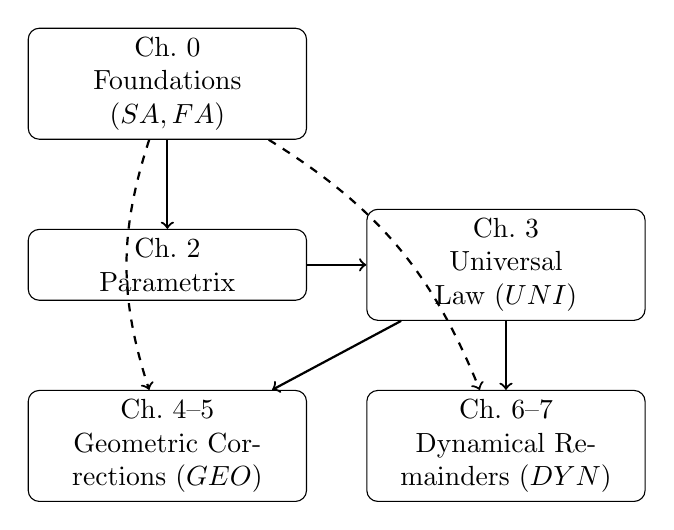
\begin{tikzpicture}[node distance=1.5cm]
\node (ch0) [draw, rectangle, rounded corners, text width=3.3cm, align=center] {Ch.~0\\Foundations\\$(SA,FA)$};
\node (ch2) [draw, rectangle, rounded corners, text width=3.3cm, align=center, below of=ch0, yshift=-0.8cm] {Ch.~2\\Parametrix};
\node (ch3) [draw, rectangle, rounded corners, text width=3.3cm, align=center, right of=ch2, xshift=2.8cm] {Ch.~3\\Universal Law $(UNI)$};
\node (ch45) [draw, rectangle, rounded corners, text width=3.3cm, align=center, below of=ch2, yshift=-0.8cm] {Ch.~4–5\\Geometric Corrections $(GEO)$};
\node (ch67) [draw, rectangle, rounded corners, text width=3.3cm, align=center, below of=ch3, yshift=-0.8cm] {Ch.~6–7\\Dynamical Remainders $(DYN)$};
\draw[->, thick] (ch0) -- (ch2);
\draw[->, thick] (ch2) -- (ch3);
\draw[->, thick] (ch3) -- (ch45);
\draw[->, thick] (ch3) -- (ch67);
\draw[->, thick, dashed] (ch0) to[bend right=18] (ch45);
\draw[->, thick, dashed] (ch0) to[bend left=18] (ch67);
\end{tikzpicture}
\caption{\textbf{Figure 1.4 (Logical architecture).} Solid arrows: primary dependence; dashed: secondary/contextual. The SA$\to$FA$\to$GEO$\to$UNI$\to$(DYN) pipeline is the backbone.}
\label{fig:monograph-structure}
\end{figure}

\paragraph{Bridges.}
The four contributions in §\ref{sec:contrib} address, one by one, the structural gaps highlighted by the four historical paradigms: (SA/FA) remedy the lack of a functional framework for interior walls; (UNI) supplies the missing local law; (GEO) organizes the first geometry–dependent corrections; (DYN) imports global refinements unavailable in purely local analyses.
Foundations (Ch.~0) $\Rightarrow$ Parametrix (Ch.~2) $\Rightarrow$ Universal law (Ch.~3) $\Rightarrow$ Geometric next order (Ch.~4–5) $\Rightarrow$ Dynamical remainders (Ch.~6–7).

\medskip

% ============================================================
% Motivation (expanded, programmatic; harmonized with Ch.~0)
% ============================================================

\section{Motivation}\label{sec:motivation}

Lithomathematics is motivated by ubiquity of phenomena, insufficiency of prior theories, and contemporary scientific demands.
It is also methodologically inevitable: the appearance of a new curvature–independent coefficient $a_\Gamma$ (Chapter~0, \textbf{Definition~\ref{def:heat-expansion}}) forces a coherent theory.

\subsection{The Phenomenology of Internal Barriers.}\label{subsec:phenomenology}
Geology (fractures/strata); materials (laminates/insulators); quantum devices (dots/billiards); engineering (acoustic/thermal shields); microfluidics/biology (impermeable membranes).
All instantiate $u|_\Gamma=0$ in the interior.

\subsection{Why classical approaches fall short.}\label{subsec:why-fall-short}
\begin{center}
\renewcommand{\arraystretch}{1.1}
\begin{tabular}{|l|l|l|l|}
\hline
\textbf{Framework} & \textbf{Object} & \textbf{Spectral law} & \textbf{Limitation} \\
\hline
Boundary geometry & $(M,\partial M)$ & $a_{1/2}\propto \vol(\partial M)$ & excludes interior partitions \\
\hline
Transmission theory & continuity/jump on $\Gamma$ & model/impedance–dependent & universality lost (coupling) \\
\hline
Robin/impedance & boundary w/ $\alpha$ & depends on $\alpha$ & extrinsic parameters dominate \\
\hline
Scattering theory & open systems & asymptotics at infinity & leakage, not confinement \\
\hline
Lithomathematics & $u|_\Gamma=0$ (internal) & $a_\Gamma\propto \vol(\Gamma)$ & universal, parameter–free \\
\hline
\end{tabular}
\end{center}

\subsection{Methodological necessity.}\label{subsec:method-necessity}
\begin{itemize}
  \item \textbf{Universality:} the existence of $a_\Gamma$ demands explanation beyond case studies (\textbf{Convention~\ref{conv:universality}}).
  \item \textbf{Simplicity:} Dirichlet slicing removes transmission diffraction and parameter dependence (cf.\ \textbf{Remark~\ref{rem:components}}).
  \item \textbf{Modularity:} SA–FA–GEO–UNI–DYN adapts to Schr\"odinger operators, multiple walls, higher–order elliptic operators.
  \item \textbf{Beyond homogenization:} unlike homogenization (averaging microstructure), lithomathematics fixes a \emph{hard wall} and extracts a \emph{local universal} contribution valid across scales.
\end{itemize}

\subsection{Applied motivations (selected).}\label{subsec:applied}
Thermal transport (area–law capacity deficit), quantum chaos/nanostructures (hard–wall confinement, altered level statistics), geophysics (energy trapping), design (barrier fingerprints).

\subsection{Contemporary scientific context.}\label{subsec:context}
Nanoscale confinement, metamaterial layering, quantum architectures rely on hard walls.
Lithomathematics supplies a parameter–free leading law and a controlled hierarchy beyond.

\subsection{Numerical verification of $a_\Gamma$ (practical note).}\label{subsec:numerics}
Compute $\Tr(e^{-\tau L_\Gamma})$ for $\tau_k\downarrow 0$ (finite–element/finite–difference with exact Dirichlet on $\Gamma$), fit
\[
\tau^{(d-1)/2}\!\left(\Tr(e^{-\tau L_\Gamma})-a_0\tau^{-d/2}\right)=A+B\tau^{1/2}+\cdots.
\]
Then $A \approx a_{1/2}(\partial M)+a_\Gamma(\Gamma)$; toggling the wall isolates $a_\Gamma$.
(Algorithmic details in Appendix~B.)

\subsection{Expected main theorems (informal; with chapter anchors).}\label{subsec:expected}
\begin{itemize}
  \item \textbf{Theorem (Universal interior law; Ch.~3).}
  For $C^2$ internal Dirichlet walls with positive reach,
  \[
  \Tr(e^{-\tau L_\Gamma}) \;=\; a_0\tau^{-d/2} \;+\; \big(a_{1/2}(\partial M)+a_\Gamma(\Gamma)\big)\tau^{-(d-1)/2} \;+\; O(\tau^{-(d-2)/2}),
  \quad
  a_\Gamma(\Gamma) \;=\; -\tfrac14(4\pi)^{-(d-1)/2}\,\vol_{d-1}(\Gamma).
  \]
  \item \textbf{Theorem (Stability; Ch.~3).}
  $a_\Gamma$ is stable under $C^2$ perturbations preserving reach/transversality (\textbf{Remark~\ref{rem:robust-coeff}}).
  \item \textbf{Theorem (Geometric next order; Ch.~4–5).}
  Coefficients at $\tau^{-(d-2)/2}$ are explicit curvature invariants; constants are controlled by $\kappa(\Gamma)$ (\textbf{Definition~\ref{def:complexity}}).
  \item \textbf{Theorem (Componentwise spectrum; Ch.~2).}
  $\Spec(L_\Gamma)=\bigsqcup_j \Spec(L^{(j)})$ and $L^2(M)\cong\bigoplus_j L^2(U_j)$ (\textbf{Remark~\ref{rem:components}}).
  \item \textbf{Theorem (Dynamical remainders; Ch.~6–7).}
  Under $H_{\mix}^{\heartsuit}$ (\textbf{Hypothesis~\ref{hyp:mixing-hermetic}}),
  \[
  N_\Gamma(\lambda) \;=\; C_d\vol(M)\lambda^{d/2} \;-\; \tfrac14 C_{d-1}\vol(\partial M\cup\Gamma)\lambda^{(d-1)/2}
  \;+\; O\!\big(\kappa(\Gamma)\lambda^{(d-2)/2-\alpha}\big).
  \]
\end{itemize}

\subsection{Prospective generalizations (research program).}\label{subsec:generalizations}
Multiple internal walls; Schr\"odinger operators $-\Delta+V$ (bounded $V$) with persistence of $a_\Gamma$; partial transmission (quantified loss of universality); random/rough walls (probabilistic robustness of the interior density); noncompact confinement (local universality vs.\ global scattering).

\subsection{Computational and Practical Aspects}\label{sec:computational}
\paragraph{Spectra of $L_\Gamma$.}
Finite–element Dirichlet discretizations on $M\setminus\Gamma$ with exact wall enforcement converge spectrally; mesh refinement is localized near $\Gamma$ to resolve the collar while preserving global balance.
\paragraph{Estimating $\kappa(\Gamma)$.}
Area is computed directly; the mean curvature $H_\Gamma$ follows from a $C^2$ surface fit on the mesh and is integrated with $L^2$ accuracy. The invariant is scale–free by construction.
\paragraph{Isolating $a_\Gamma$.}
Wall–toggle experiments and short–time fits of $\Tr(e^{-\tau L_\Gamma})$ separate interior from exterior surface contributions, validating the universal density $-\frac14(4\pi)^{-(d-1)/2}$.

\subsection{Fundamental Problems and Open Questions}\label{sec:open-questions}
\begin{enumerate}
  \item \textbf{Universality under minimal geometry.} Determine the weakest regularity and reach assumptions ensuring the interior surface density $-\tfrac14(4\pi)^{-(d-1)/2}$.
  \item \textbf{Sharp complexity control.} Identify regimes where $\kappa(\Gamma)$ yields best–possible exponents or constants in remainders, and characterize their optimality.
  \item \textbf{Inverse lithomathematics.} Quantify how $\Spec(L_\Gamma)$ constrains $\Gamma$ up to isometry (stability, obstructions, nonuniqueness).
  \item \textbf{Topology via spectrum.} Clarify the Morse–theoretic and lithotopological information encoded in $\Spec(L_\Gamma)$ for the partitioned manifold $M\setminus\Gamma$.
\end{enumerate}

\subsection{The Lithomathematical Roadmap: 2025–2035}\label{subsec:roadmap}
\begin{enumerate}
  \item \textbf{Phase I (Foundations, 2025–2028).} Universal law for rough walls ($C^{1,1}$); magnetic/Schr\"odinger extensions; reference implementations for numerical lithomathematics.
  \item \textbf{Phase II (Inverse Problems, 2028–2032).} Spectral reconstruction of $\Gamma$ (lithotomography); stability and uniqueness regimes; algorithms and benchmarks.
  \item \textbf{Phase III (Generalized Lithostructures, 2032–2035).} Random/stochastic walls; graph and network analogues; noncommutative lithomathematics on partitioned operator algebras.
\end{enumerate}

\subsection{Narrative bridge.}\label{subsec:narrative}
Foundations (Ch.~0) $\to$ Parametrix (Ch.~2) $\to$ Universal law (Ch.~3) $\to$ Geometric next order (Ch.~4–5) $\to$ Dynamical remainders (Ch.~6–7) $\to$ Applications/Models (Appendices).

\paragraph{Summary.}
Lithomathematics elevates internal Dirichlet walls from neglected constraints to \emph{first–class spectral objects} governed by a universal interior law, with a scale–free complexity control and an optional dynamical accelerator—precisely as formalized in Chapter~0 and developed in the parts that follow.

% ------------------------------------------------------------
% End of Chapter 1
% ------------------------------------------------------------
